\documentclass[12pt,letterpaper]{article}
\usepackage{fullpage}
\usepackage{lipsum}
\usepackage{graphicx}
\begin{document}
\title{The Eh-P's: Beam Line for Schools Proposal}
\author{
Ryan Marks\\
Jiarui Pu \\ 
Andrew Tan\\
Eric Ye\\
\\
Mentor: Mr. Henri van Bemmel\\
\normalsize{\texttt{hmvb15@rogers.com}}
}

\date{\today}
\maketitle
\section{Proposed Experiments}
The goal of these experiments is to investigate the properties of charged particle beams as currents.

\subsection{Experiment 1}
The first experiment will be affected in order to verify that a stream of particles do function as currents.
This experiment will use a beam of charged particles running through a ring of magnetic field detectors.
If the charged beam does function as a current it will produce a magnetic field around the beam.

\subsection{Experiment 2}
If the first experiment does produce a magnetic field we will be able to move on the next experiment.
This experiment will effectively verify the Hall Effect with particle beams. 
A wire will be suspended and will have a fixed current running adjacent to the particle beam.
The particle beam will be fired through the six pane telescope in order to observe deflection due to the produced B-field.

\subsection{Experiment 3}
\label{experiment_setup3}
\begin{figure}[h]
  \centering
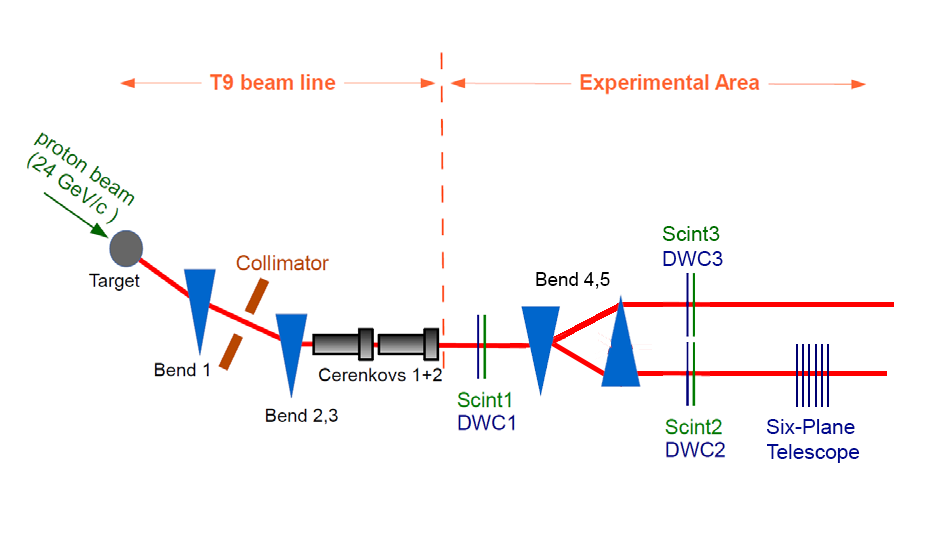
\includegraphics[]{experimental_setup3.png}
 \caption{The proposed beam line arrangement for experiment 3.}
\end{figure}


The final experiment will use an initial beam of particles with opposite charges, and by running it through two adjacent, equal, but oppositely directioned B-fields.
This will produce two particle beams with opposite currents. 
This should cause the particle beams to deflect one another if they have enough magnitude to defeat the electrostatic attraction.

\end{document}
